\documentclass[10pt]{article}
\usepackage{icmlko}

\icmlmeta{IP 파운데이션 월드모델}{114}{이름이 달라도 된다}{매장 노출은 아홉 도메인에서 제작자 이력이고 팝업에서 매장의 급인데 --- 바꿔도, 보존해도, 빼도 전부 진다}

\begin{document}

\twocolumn[
\icmlheader

\begin{abstract}
노트 113이 단서를 남겼다 --- 매장 노출 잔차가 아홉 출처 중 일곱에서 1을
넘는다. 정의를 읽으니 이유가 명백했다. \textbf{아홉 도메인은 전부 ``제작자 ·
제작사 · 출판사 · 퍼블리셔의 사전 작품 건수''이고 팝업만 ``사람이 매긴 매장의
급''}(더현대 · 성수 같은 자리)이다. \textbf{이름만 같고 다른 것을 잰다.}
그리고 팝업에는 진짜 대응물이 있다 --- 같은 IP 의 사전 팝업 이력
(\texttt{prior\_label\_n\_log} 등). 고쳐 봤다. \textbf{세 가지 고침이 전부
진다.} ① 사전 이력으로 바꾸면 판정치 $-$0.0066 · 팝업 $-$0.0639이고
\textbf{잔차마저 0.814에서 0.846으로 나빠진다.} ② 바꾸되 매장 급을 고유 축으로
보존해도 $-$0.0020 · $-$0.0190. ③ 정렬에서 아예 빼면 \textbf{악화 4/4}
($-$0.0115, 구간 넷 다 0 아래)이고 열 대상 중 아홉이 잃는다(모바일 $-$0.047 ·
아이돌 $-$0.021). 유일하게 잔차를 낮추는 것(팝업에서만 끄기, 0.814$\to$0.689)은
성적을 거의 안 바꾼다($-$0.0005 · $-$0.0010). \textbf{결론은 하나다 --- 이름이
달라도 된다.} 프로크루스테스가 맞추는 것은 개념이 아니라 기하다. 매장의 급과
제작자 이력은 개념이 달라도 각 도메인 안에서 같은 자리를 차지한다 --- 둘 다
``이 작품 뒤에 얼마나 큰 것이 서 있나''의 대리다. 이 프로젝트에서 \textbf{원리적으로
옳은 쪽이 지는 여섯째 사례}다(노트 40 · 48 · 85--88 · 103 · 105, 그리고 여기).
\end{abstract}
]

\begin{figure*}[t]
\centering
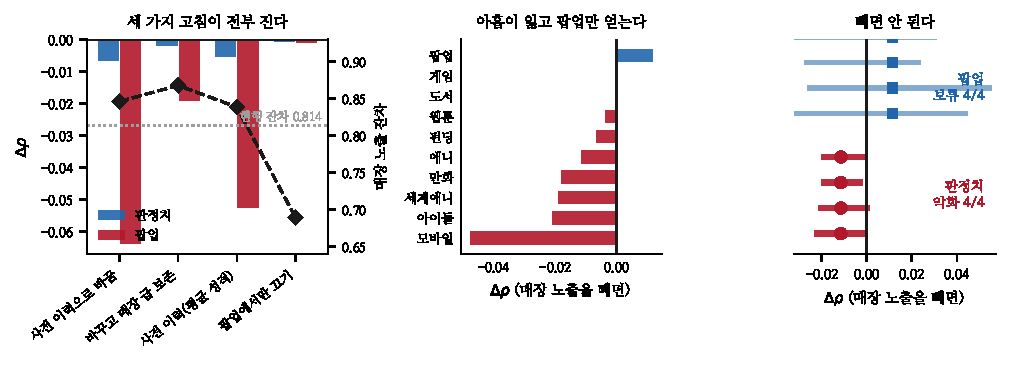
\includegraphics[width=\textwidth]{figs/nd.pdf}
\caption{왼쪽 --- 세 가지 고침이 전부 진다. 가운데 --- 아홉이 잃고 팝업만
얻는다. 오른쪽 --- 빼면 안 된다.}
\end{figure*}

\section{이름만 같은 축이 맞다}

\begin{table}[t]
\centering\tsize
\caption{매장 노출이 도메인마다 실제로 재는 것.}
\begin{tabular}{ll}
\toprule
모바일 & 개발사 사전 출시 건수 \\
웹툰 & 작가 사전 연재 건수 \\
만화 & 작가 사전 작품 건수 \\
세계애니 & 제작사 사전 작품 건수 \\
게임 & 퍼블리셔 사전 출시 건수 \\
도서 & 동일 출판사 사전 출간 건수 \\
펀딩 & 동일 창작자 사전 프로젝트 건수 \\
아이돌 & 사전 데뷔 건수 \\
\midrule
\textbf{팝업} & \textbf{사람이 매긴 매장의 급} \\
\bottomrule
\end{tabular}
\end{table}

아홉은 \emph{만든 사람이 전에 몇 개 만들었나}이고 팝업은 \emph{어느 자리에서
여나}다. 노트 74의 법칙(``이름이 같다고 같은 것을 재는 것이 아니다'')이 남은
공통 축에서 마지막으로 확인된다.

\begin{table}[t]
\centering\tsize
\caption{팝업에 있는 후보들. 사전 이력이 진짜 대응물이다.}
\begin{tabular}{lrr}
\toprule
& 덮개율 & 라벨 상관 \\
\midrule
\textbf{매장 노출}(현행, 사람이 매김) & 100\% & \textbf{$+$0.348} \\
\midrule
직전작 건수 & 100\% & $+$0.154 \\
직전작 평균 성적 & 100\% & $+$0.138 \\
사전 팝업 수 & 100\% & $+$0.026 \\
매장 급(자동) & 100\% & $-$0.159 \\
\bottomrule
\end{tabular}
\end{table}

\section{세 가지 고침이 전부 진다}

\begin{table}[t]
\centering\tsize
\caption{$\Delta$. 현행은 판정치 $+$0.4270 · 팝업 $+$0.4601 · 잔차 0.814.}
\begin{tabular}{lrrr}
\toprule
& 판정치 & 팝업 & 잔차 \\
\midrule
① 사전 이력(건수)으로 바꿈 & $-$0.0066 & $-$0.0639 & \textbf{0.846} \\
② 바꾸고 매장 급은 고유 축으로 & $-$0.0020 & $-$0.0190 & 0.868 \\
③ 사전 이력(평균 성적)으로 & $-$0.0053 & $-$0.0524 & 0.839 \\
④ 팝업에서만 끄기 & $-$0.0005 & $-$0.0010 & \textbf{0.689} \\
\bottomrule
\end{tabular}
\end{table}

\claimx{\textbf{개념을 바로잡아도 잔차가 안 내려간다.} 사전 이력으로 바꾸면
개념은 아홉과 같아지는데 잔차가 0.814에서 0.846으로 \emph{올라간다}. 개념
정합이 기하 정합을 만들지 않는다.}{정보를 보존한 ②도 잔차가 0.868로 가장
나쁘다. 축이 하나 늘어 인자 공간이 희석되는 노트 102의 효과가 섞였을 수 있다.}

\section{빼도 안 된다}

\begin{table}[t]
\centering\tsize
\caption{매장 노출을 정렬에서 뺀다. 씨앗 넷 · 붓스트랩 80회.}
\begin{tabular}{lrl}
\toprule
& $\Delta$ & 95\% 구간 \\
\midrule
판정치 & $-$0.0115 & $-$0.0220 $\sim$ $-$0.0008 \quad \textbf{악화} \\
& & $-$0.0201 $\sim$ $-$0.0002 \quad \textbf{악화} \\
& & $-$0.0188 $\sim$ $-$0.0029 \quad \textbf{악화} \\
& & $-$0.0187 $\sim$ $-$0.0011 \quad \textbf{악화} \\
팝업 & $+$0.0116 & 보류 4/4 \\
\bottomrule
\end{tabular}
\end{table}

\begin{table}[t]
\centering\tsize
\caption{대상별. 매장 노출을 빼면.}
\begin{tabular}{lrr}
\toprule
& 현행 & $\Delta$ \\
\midrule
모바일 & $+$0.631 & \textbf{$-$0.047} \\
아이돌 & $+$0.479 & $-$0.021 \\
세계애니 & $+$0.528 & $-$0.019 \\
만화 & $+$0.529 & $-$0.018 \\
애니 & $+$0.313 & $-$0.011 \\
펀딩 & $+$0.215 & $-$0.007 \\
웹툰 & $+$0.480 & $-$0.003 \\
도서 · 게임 & & $\pm$0.000 \\
\midrule
\textbf{팝업} & $+$0.460 & \textbf{$+$0.012} \\
\bottomrule
\end{tabular}
\end{table}

\claimx{매장 노출은 \textbf{이름이 달라도 값을 한다.} 빼면 판정치가 악화 4/4이고
열 대상 중 아홉이 잃는다. 팝업 하나만 $+$0.012 얻는데 보류다.}{팝업만 이득인
것은 팝업이 개념 불일치의 당사자이기 때문일 수 있다. 다만 $+$0.012 가 보류라
근거로 삼을 수 없다.}

\begin{quote}\fontsize{9.5}{11.5}\selectfont
\textbf{프로크루스테스가 맞추는 것은 개념이 아니라 기하다.} 매장의 급과
제작자 이력은 개념이 달라도 각 도메인 안에서 같은 자리를 차지한다 --- 둘 다
``이 작품 뒤에 얼마나 큰 것이 서 있나''의 대리이고, 그것이 다른 축들과 맺는
관계가 도메인마다 비슷하다. \textbf{정렬에 필요한 것은 같은 개념이 아니라
같은 관계다}(Meredith 1993의 형태 불변).
\end{quote}

\section{여섯 번째로 원리가 졌다}

\begin{table}[t]
\centering\tsize
\caption{``원리적으로 옳은 쪽이 진다''의 목록.}
\begin{tabular}{ll}
\toprule
노트 40 & 전역 정렬 $\to$ 쌍별 정렬 \\
노트 48 & $\lambda$ 겹침 규칙 $\to$ 1.0 고정 \\
노트 85--88 & 공유 인코더 $\to$ 프로크루스테스 \\
노트 103 & 새 축을 공통 슬롯으로 승격 \\
노트 105 & 입장료의 개념 정리(가격 아닌 것 끄기) \\
\textbf{노트 114} & \textbf{매장 노출의 개념 정리} \\
\bottomrule
\end{tabular}
\end{table}

\claimx{여섯 번 모두 같은 모양이다 --- \textbf{개념을 바로 세우면 성적이 내린다.}
모형이 붙잡고 있는 것은 사람이 붙인 이름이 아니라 자료 안의 관계다.}
{여섯 사례 중 셋(103 · 105 · 114)은 최근 열두 노트에 몰려 있다. 최근에
개념 정리를 많이 시도해서일 뿐 법칙이 강해진 것은 아니다.}

\section{한계}

\begin{itemize}[leftmargin=1.1em,itemsep=0.15em]
\item \textbf{바꿀 것이 없다.} 네 설정이 전부 현행보다 나쁘거나 같다.
\item 팝업의 사전 이력 후보를 넷만 봤다. 조합(건수 $\times$ 평균 성적)은
      안 해 봤다.
\item ``같은 관계''를 정량화 못 했다. 적재의 다른 축들과의 각도를 재면
      될 것인데 안 했다.
\item 팝업이 $+$0.012 얻는 것을 설명 못 한다.
\item 이제 공통 축 다섯이 전부 검토됐다. 남은 미검토 설정이 없다.
\end{itemize}

\section{다음}

\begin{enumerate}[leftmargin=1.3em,itemsep=0.15em]
\item \textbf{``같은 관계''를 잰다} --- 각 도메인에서 축이 다른 축들과 맺는
      각도를 재고, 그 각도의 일치가 잔차를 예측하는지 본다. 그러면 새 축을
      \emph{긁기 전에} 고르는 기준이 처음으로 생긴다(노트 101 · 104가 두 번
      실패한 그 기준).
\item \textbf{팝업 레코드} --- 여덟 노트가 같은 곳을 가리킨다. 25건이면 방향,
      510건이면 설계. \textbf{모으는 절차를 설계한다.}
\item 텀블벅 API --- 펀딩만 미디어 홍보 0\%다.
\item 공통 축 다섯이 다 검토됐으니 \textbf{여섯째를 찾는 판을 다시 연다} ---
      이번에는 ``같은 관계'' 기준으로.
\end{enumerate}

\vspace{0.6em}
\hrule height 0.3pt
\vspace{0.5em}
{\footnotesize
\textbf{참고문헌}\\[0.3em]
Meredith, W. (1993). Measurement invariance, factor analysis and factorial
invariance. \emph{Psychometrika}, 58(4), 525--543.\\[0.15em]
Schoenemann, P. H. (1966). A generalized solution of the orthogonal Procrustes
problem. \emph{Psychometrika}, 31(1), 1--10.\\[0.15em]
Gower, J. C., Dijksterhuis, G. B. (2004). \emph{Procrustes Problems}.
Oxford University Press.\\[0.15em]
Ben-David, S. et al. (2010). A theory of learning from different domains.
\emph{Machine Learning}, 79(1--2), 151--175.\\[0.15em]
Efron, B., Tibshirani, R. J. (1993). \emph{An Introduction to the Bootstrap}.
Chapman \& Hall.
}

\end{document}
